\documentclass[../main.tex]{subfiles}

\begin{document}
	\section{Light}
	\begin{preamb}
		Light can be studied as a wave. In this chapter we will look at how light interacts with matter.
	\end{preamb}
	
	\subsection{Reflection}
	
	\pdef{Normal}{The normal is an imaginary line draw perpendicular to the surface that reflection is taking place at.}
	
	\pdef{Angle of Incidence}{The angle of incidence is the angle between the incident ray and the normal.}
	
	\pdef{Angle of Reflection}{The angle of reflection is the angle between the reflected ray and the normal.}
	
	\begin{center}
		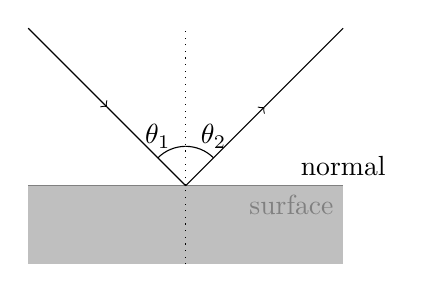
\begin{tikzpicture}
			\draw [color=gray] (-2,0) -- (2,0) node [anchor=north east] {surface};
			\node [anchor=south] at (2,0) {normal};
			\fill [color=gray, fill opacity=0.5] (-2,-1) -- (-2,0) -- (2,0) -- (2, -1);
			\draw [dotted] (0,-1) -- (0,2);
			\draw [->] (-2,2) -- (-1,1);
			\draw (-1,1) -- (0,0);
			\draw (0,0.5) arc (90:135:0.5) node [anchor=south] {\(\theta_1\)};
			\draw (0,0.5) arc (90:45:0.5) node [anchor=south] {\(\theta_2\)};
			\draw [->] (0,0) -- (1,1);
			\draw (1,1) -- (2,2);
		\end{tikzpicture}
	\end{center}
	
	\pdef{First Law of Reflection}{The incident ray, reflected ray, and the normal lie on the same plane.}
	
	\pdef{Second Law of Reflection}{In reflection, the angle of incidence is equal to the angle of reflection. \[\theta_1 = \theta_2\]}
	I have chosen to name the angles \(\theta_1\) and \(\theta_2\) due to the reversible nature of light. It does not matter which way the light goes; the angles will be preserved.
	
	\subsection{Refraction}
	
	\subsubsection{Essentials}
	
	\pdef{Angle of Refraction}{The angle of refraction is the angle between the refracted ray and the normal.}
	
	\begin{center}
		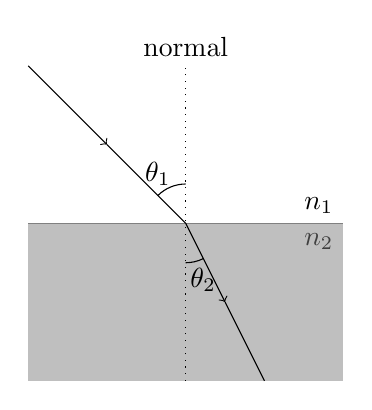
\begin{tikzpicture}
			\node [anchor=south east] at (2,0) {\(n_1\)};
			\node [anchor=north east] at (2,0) {\(n_2\)};
			\draw [color=gray] (-2,0) -- (2,0);
			\fill [color=gray, fill opacity=0.5] (-2,-2) -- (-2,0) -- (2,0) -- (2,-2);
			\draw [dotted] (0,-2) -- (0,2) node [anchor=south] {normal};
			\draw [->] (-2,2) -- (-1,1);
			\draw (-1,1) -- (0,0);
			\draw (0,0.5) arc (90:135:0.5) node [anchor=south] {\(\theta_1\)};
			\draw (0,-0.5) arc (270:296:0.5) node [anchor=north] {\(\theta_2\)};
			\draw [->] (0,0) -- (0.5,-1);
			\draw (0.5,-1) -- (1,-2);
		\end{tikzpicture}
	\end{center}
	
	\pdef{First Law of Refraction}{The incident ray, reflected ray, and the normal lie on the same plane.}
	
	\pdef{Second Law of Refraction}{The second law of refraction (also known as Snell's Law) states that for two given media, the ratio of the sine of the angle of incidence to the sine of the angle of refraction is a constant.}
	
	\peqn{Refractive Index}{The refractive index of a medium is the ratio of the speed of light in vacuum to the speed of light in the medium}{n = \frac{c}{v}}
	Sometimes it might also be \[ n = \frac{\text{real depth}}{\text{apparent depth}}\].
	
	\peqn{Snell's Law}{Snell's Law is the same thing as the second law of refraction, mathematically expressed as}{n_1 \sin \theta_1 = n_2 \sin \theta_2}
	
	\pdef{Critical Angle}{The critical angle is defined as the angle of incidence in an optically denser medium for which the angle of refraction in the optically less dense medium is \SI{90}{\degree}.}
	
	\pdef{Total Internal Reflection}{Total internal reflection is the complete reflection of a light ray inside an optically denser medium at its boundary with an optically less dense medium.}
	
	\begin{center}
		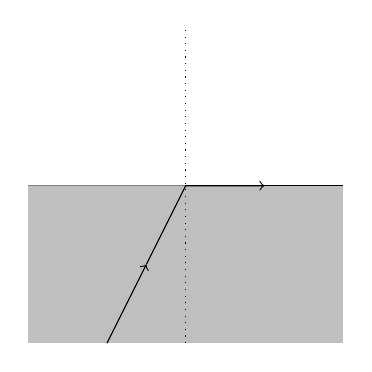
\begin{tikzpicture}
			\draw [color=gray] (-2,0) -- (2,0);
			\fill [color=gray, fill opacity=0.5] (-2,-2) rectangle (2,0);
			\draw [dotted] (0,-2) -- (0,2);
			\draw [->] (-1,-2) -- (-0.5,-1);
			\draw [->] (-0.5,-1) -- (0,0) -- (1,0);
			\draw (1,0) -- (2,0);
		\end{tikzpicture}
	\end{center}
	
	\subsubsection{Lenses}
	Lenses are cool and I'm a bit lazy to write this chapter, maybe later.
\end{document}
